\chapter{Ergebnisse}

\section{Laufzeit}


Um die verschiedenen Methoden zu vergleichen wurden verschiedene Tests durchgeführt.
Als erstes wurde die Laufzeit der einzelnen Verfahren verglichen. 
Hierzu wird von der \emph{clock\_gettime} Funktion gebraucht gemacht. Diese liefert einen \emph{struct} aus dem die zeit bis auf Nanosekunden-Genauigkeit ausgelesen werden kann.
Es wurden folgende Laufzeiten für jeden Algorithmus ermittelt:
\begin{itemize}
\item Extraktion der Merkmale
\item Matching der Deskriptoren
\item Berechnung der Homographie
\item Gesamte Bearbeitung eines Frames
\end{itemize}

Die für den ersten Punkt benötigte Zeit ist stark von der gewählten Methode abhängig. 
Die Matching-Zeit hängt zum einem von dem Deskriptortyp ab und zum anderen ist diese sehr von der Umgebung bestimmt da sie von der Anzahl der Merkmale abhängt.
Die Laufzeit der Homographie-Bestimmung hängt auch von der Merkmalsanzahl ab.

In Volgender Tabelle sind die Durchnittlichen Laufzeiten aufgelistet. Diese wurden bei der Bearbeitung eines Testvideos ermittelt.

\begin{center}
    \begin{tabular}{ c | C | C | C | C |}
      & Extraktion & Matching & Homographie & Gesamt\\ \hline
    SIFT & 370 & 90 & 2 & 495 \\ \hline
    SURF & 111 & 47 & 2 & 184 \\ \hline
    ORB & 17 & 25 & 6 & 64 \\
    \hline
    \end{tabular}
\end{center}


\section{Anzahl der korrekten Matches}

Als weiteres Testkriterium wurde die Anzahl der richtig zugewiesenen Merkmale bestimmt.
Hierzu wurde von der Bitmaske die von \emph{findHomography} zurückgegeben wird Gebrauch gemacht. Aus dieser können die tatsächlich von der Funktion verwendeten Matches bestimmt werden. Die gefundenen Matches passen somit in die Gesamtkonstellation und werden als richtig eingestuft.
Um möglichst aussagekräftige Ergebnisse zu erhalten wurden 40 sekündige Videos der Testobjekte aufgenommen und anschließend die durchschnittlichen Korrekten Matches für jeden Algorithmus berechnet. Um unvorhersehbare Effekte beim Startvorgang des Programms auszuschließen wurden für die Mittelwerte nur Matches ab der 10. Sekunde berücksichtigt.


\begin{center}
    \begin{tabular}{ c | C | C | C | C | C |}
      & Kork & Müsli & Tomatendose & Kirschglas & Spardose \\ \hline
    SIFT & 80 & 298 & 181 & 161 & 46 \\ \hline
    SURF & 11 & 149 & 80 & 78 & 17 \\ \hline
    ORB & 26 & 156 & 110 & 170 & 59 \\
    \hline
    \end{tabular}
\end{center}

Wie erwartet schneiden die Merkmale die von einem SIFT-Deskriptor beschrieben werden bei der Wiedererkennung am besten ab.
Bei 3 von den 5 Testobjekten werden deutlich mehr Merkmale korrekt wiedererkannt als bei den anderen beiden Methoden.
Allerdings werden bei den schwerer zu erkennenden Objekten anhand des ORB-Deskriptors mehr Merkmale richtig zugeordnet.
SURF liefert in diesem Test für alle 5 Objekte das schlechteste Ergebnis.

\section{Stabilität gegen Rotation}

Beim zweiten Vergleich wurde getestet wie rotationsinvariant die Algorithmen sind.
Hierzu wurde jedes Objekt soweit gedreht bis keine eindeutige Lokalisierung mehr möglich war.
Hierbei wurde darauf geachtet dass bei den Vergleichen die Position der Kamera konstant blieb und die Objekte nur um ihre senkrechte Achse gedreht wurden.
Nachdem die maximale Rotation erreicht wurde, wurde der Winkel gemessen und auf 5 Grad gerundet, da eine genauere Messung mit den vorhandenen Mitteln nicht möglich war.

\begin{center}
    \begin{tabular}{ c | C | C | C | C | C |}
      & Kork & Müsli & Tomatendose & Kirschglas & Spardose \\ \hline
    SIFT & 55 & 60 & 55 & 65 & 35 \\ \hline
    SURF & 45 & 55 & 50 & 45 & 35 \\ \hline
    ORB & 45 & 45 & 30 & 55 & 25 \\
    \hline
    \end{tabular}
\end{center}

Auch hier liefert SIFT die besten Ergebnisse, selbst bei den schwerer zu erkennenden Objekten, obwohl bei diesen weniger Merkmale als bei ORB korrekt zugeordnet wurden.
Auch SURF ist trotz der wesentlich geringeren Menge an Merkmalen im schnitt besser als ORB.

\section{Stabilität gegen Skalierung}

Eine weitere wichtige Eigenschaft der Merkmale ist die Skalierungsinvarianz.
Diese führt dazu dass Objekte auch erkannt werden wenn sie kleiner oder größer (weiter oder weniger weit entfernt) als auf dem Modellbild sind.
Da die SURF und ORB Implementierungen von OpenCV nicht mit kleinen Bildern funktionieren, und die Modellbilder somit nicht runterskaliert werden konnten, war es nicht möglich die Erkennung von Objekten die größer als ihr Modellbild sind zu testen.
Da in der Praxis die zu erkennenden Objekte aber kleiner als deren Modellbilder sind, stellt dies aber kein wirkliches Problem da.
Um die Algorithmen auf die Fähigkeit kleinere Exemplare der Ojekte wiederzuerkennen zu testen, wurde die maximale Distanz von der Kamera zum Objekt gemessen bei der dieses noch korrekt erkannt werden konnte.

\begin{center}
    \begin{tabular}{ c | C | C | C | C | C |}
      & Kork & Müsli & Tomatendose & Kirschglas & Spardose \\ \hline
    SIFT & 50 & 265 & 120 & 110 & 70 \\ \hline
    SURF & 25 & 140 & 65 & 70 & 50 \\ \hline
    ORB & 30 & 125 & 45 & 50 & 40 \\
    \hline
    \end{tabular}
\end{center}

Wie bei den vorherigen Tests schnitt SIFT mit Abstand am besten ab und schaffte es, für die Verhältnisse (Consumer Grade Webcam mit VGA Auflösung), Objekte aus einer sehr großen Entfernung zu erkennen.
SURF schnitt bei allen Objekten außer dem Korkuntersetzter besser als ORB ab.

\section{Stabilität der Lokalisierung}

Ein weiteres Maß für die Güte der verschiedenen Extraktionsverfahren ist die Abweichung der Lokalisierung von der Istposition der Objekte.
Genauer ist hier die quadratische mittlere Abweichung, die Varianz, von Bedeutung.
Um diese zu ermitteln wurde auch hier ein Testvideo erstellt um gleiche Bedingungen zu gewährleisten.
Es wurde ein Histogramm von der Verteilung der X-Koordinate, der Y-Koordinate und dem Ausrichtungswinkel in Form eines Vectors erstellt.
Die als \emph{•}{csv}-Datei aus dem Programm exportierten Daten wurden mittels Gnuplot als Graphen dargestellt.
Die Verteilungen sind in den folgenden drei Graphen zu sehen, hierbei ist links die Rotation zu sehen und rechts davon die Trasnlation in x und y Richtung.
Die Translation ist jeweils in Pixeln angegeben, dies ist auch die Einheit der Zahlen auf den Achsen.
Die Rotation ist hingegen in Grad bemessen und wurde im Vergleich der angeschriebenen Zahlen gestreckt.

\begin{center}
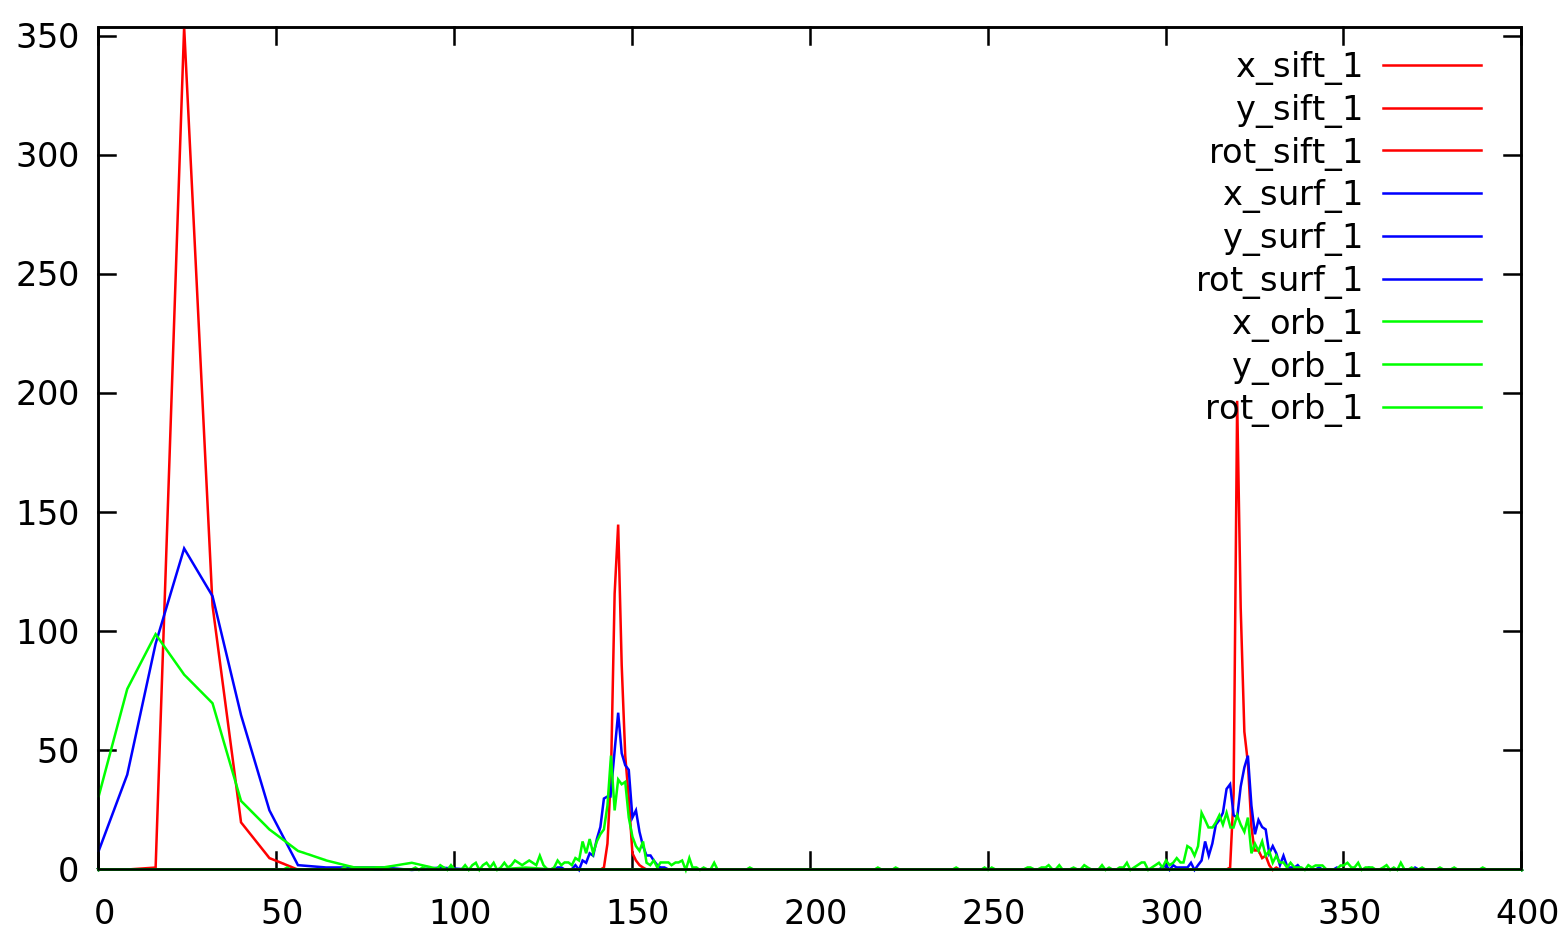
\includegraphics[width=0.75\textwidth]{verteilung1.png}

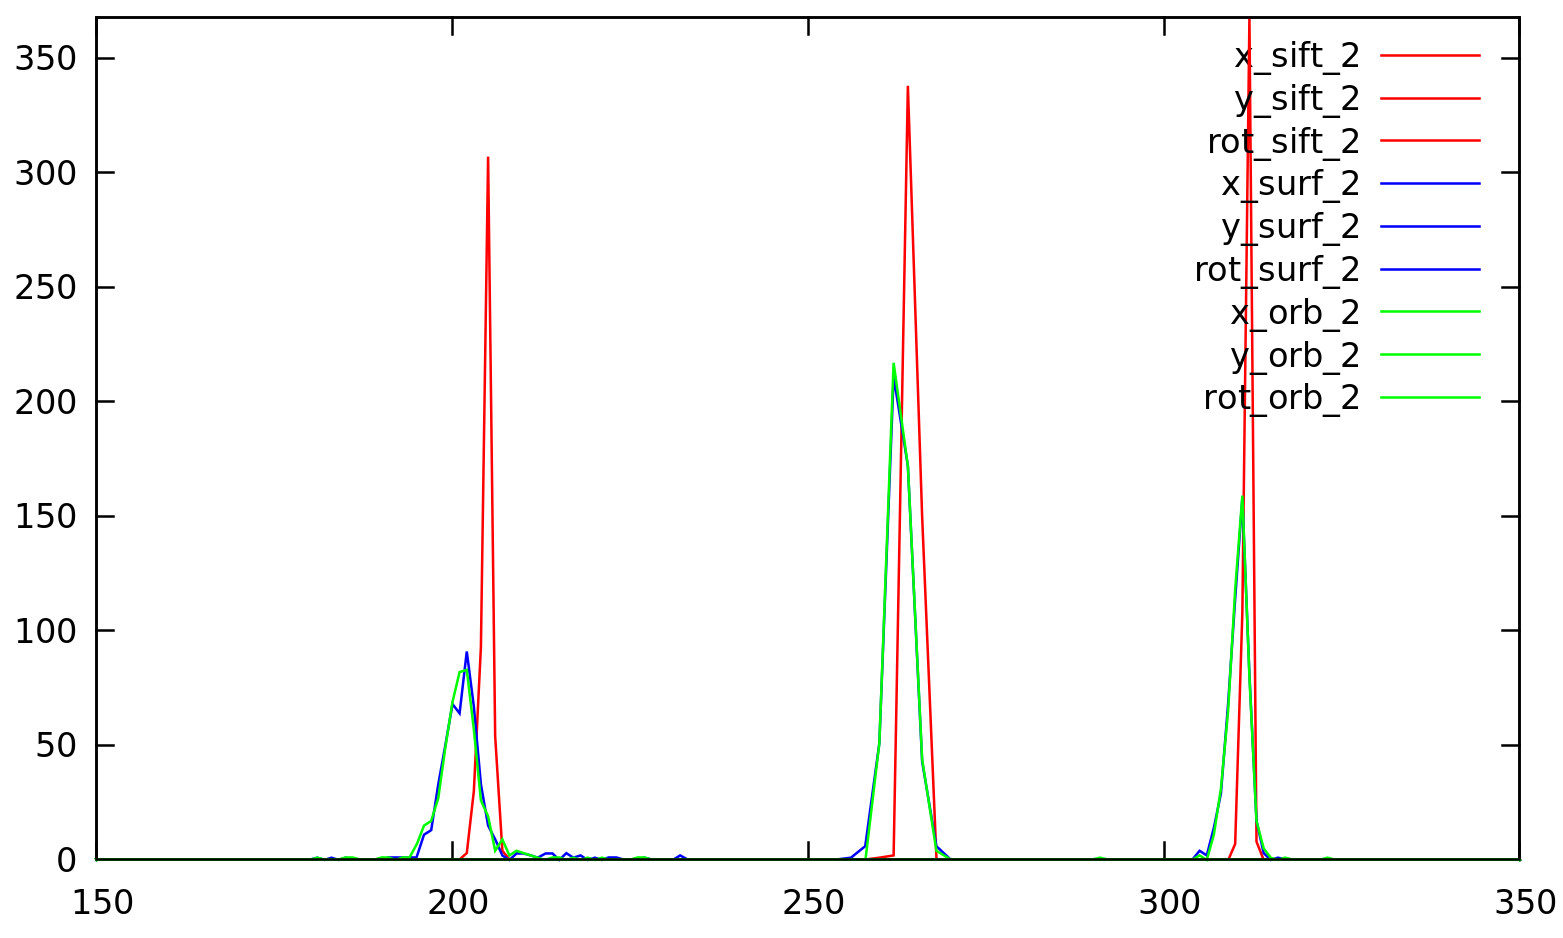
\includegraphics[width=0.75\textwidth]{verteilung2.png}

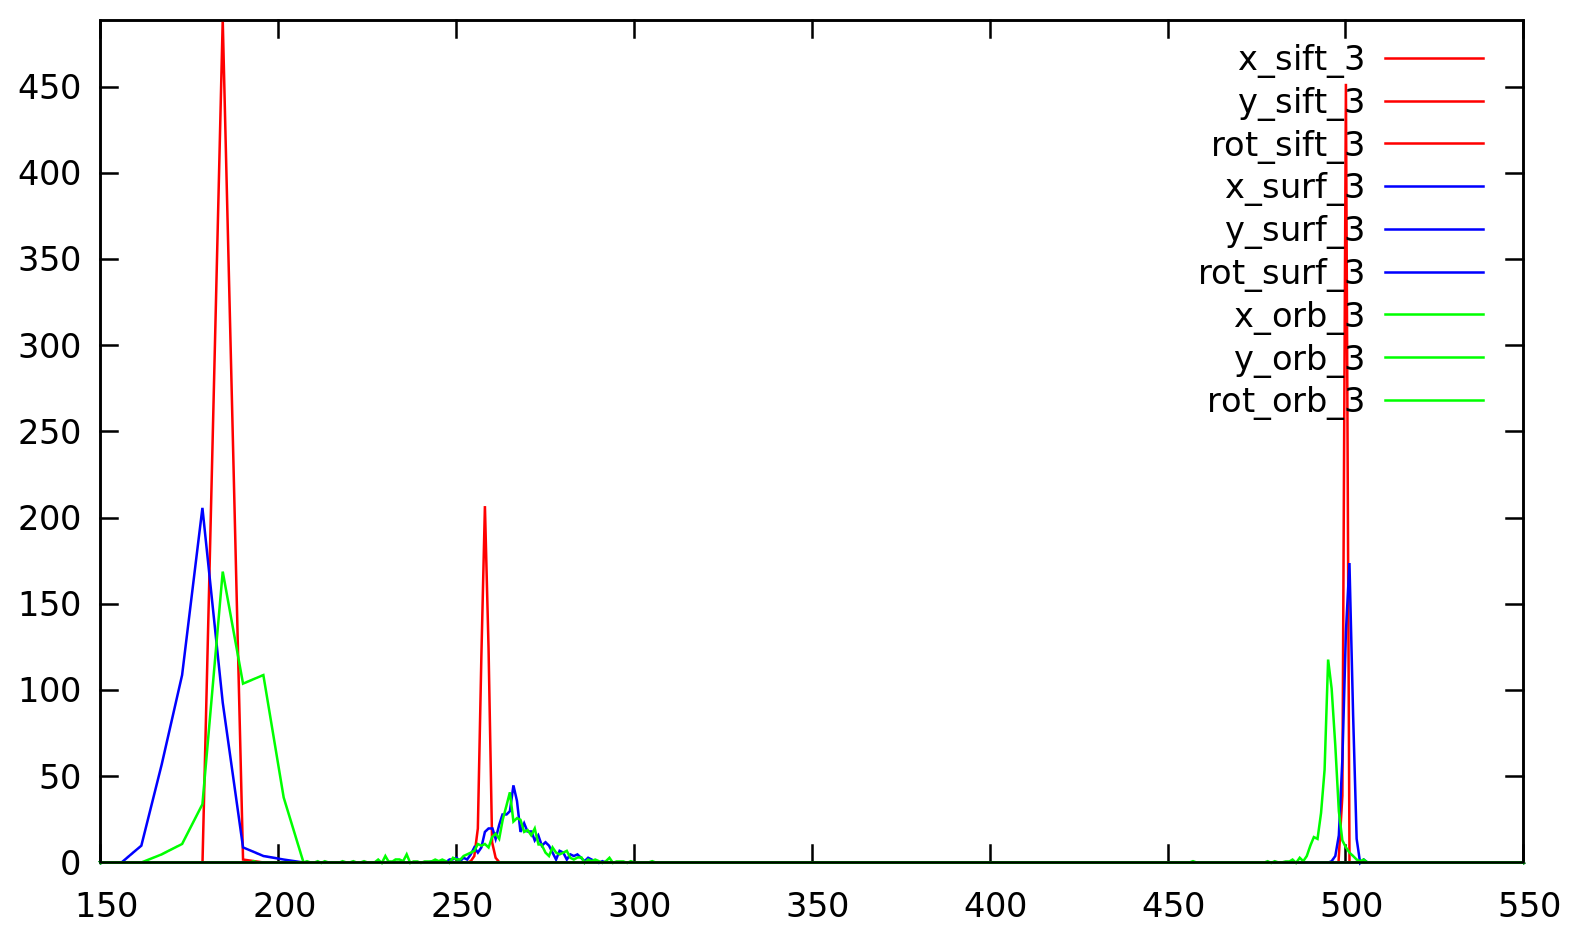
\includegraphics[width=0.75\textwidth]{verteilung3.png}
\end{center}


Wie zu erwarten da dies auch anhand der Videoausgabe des Programms deutlich sichtbar ist, zeigen die Graphiken deutlich dass die Lokalisierung durch den SIFT Algorithmus wesentlich stabiler als bei den anderen beiden Varianten ist.
SURF lokalisiert die Objekte mit größerer Genauigkeit als ORB, hat hierbei aber nur einen mäßigen Vorteil.
Man sieht dass die Verteilungen in Einigen Fällen einer summe mehrerer Normalverteilungen entsprechen. 
Dies kommt daher dass mehr als eine Konstellation an Merkmalen dem Modell ähnlich sind und somit durch die Störeinflüsse manchmal eine vollkommen falsche Position ausgegeben wird.

\section{Testvideos}

Der letzte Vergleich wurde anhand von zwei Testvideos gemacht.
Diese beinhalten die 5 Beispielgegestände in zwei verschiedenen Anordnungen.
Die Leistung der 3 Algorithmen wurde die Anzahl der Frames in welchen die Objekte erkannt wurden bestimmt.
Da es bei der gleichzeitigen Verwendung von mehreren Objekten leichter zu Fehlerkennungen kommt wurden nur Frames in denen ein Objekt mit mindestens 5 Matches erkannt wurde gezählt. 
Dies führt dazu dass es zu so gut wie keiner Fehlzuweisung kommt (weniger als 5 pro Video beobachtbar).
In folgender Tabelle sind die Anzahlen der Frames des ersten Testvideos in denen die jeweiligen Objekte gefunden wurden aufgelistet:

\begin{center}
    \begin{tabular}{ c | C | C | C | C | C |}
      & Kork & Müsli & Tomatendose & Kirschglas & Spardose \\ \hline
    SIFT & 268 & 415 & 392 & 212 & 203 \\ \hline
    SURF & x & 400 & 366 & 162 & 77 \\ \hline
    ORB & x & 370 & 342 & 150 & 56 \\
    \hline
    \end{tabular}
\end{center}

Es folgen die Frames des zweiten Videos:

\begin{center}
    \begin{tabular}{ c | C | C | C | C | C |}
      & Kork & Müsli & Tomatendose & Kirschglas & Spardose \\ \hline
    SIFT & 300 & 793 & 517 & 669 & 696 \\ \hline
    SURF & x & 695 & 285 & 548 & 443 \\ \hline
    ORB & 2 & 531 & 123 & 341 & 114 \\
    \hline
    \end{tabular}
\end{center}

Zusätzlich wurden die durchschnittlichen Zuweisungen die zu der Erkennung der Objekte geführt haben berechnet.
Erstes Video:

\begin{center}
    \begin{tabular}{ c | C | C | C | C | C |}
      & Kork & Müsli & Tomatendose & Kirschglas & Spardose \\ \hline
    SIFT & 17 & 124 & 40 & 31 & 11 \\ \hline
    SURF & x & 48 & 10 & 10 & 5 \\ \hline
    ORB & x & 66 & 11 & 11 & 9 \\
    \hline
    \end{tabular}
\end{center}

Zweites Video:

\begin{center}
    \begin{tabular}{ c | C | C | C | C | C |}
      & Kork & Müsli & Tomatendose & Kirschglas & Spardose \\ \hline
    SIFT & 9 & 65 & 22 & 44 & 26 \\ \hline
    SURF & x & 20 & 7 & 13 & 11 \\ \hline
    ORB & 6 & 23 & 9 & 14 & 18 \\
    \hline
    \end{tabular}
\end{center}

Wie nach den vorherigen Tests zu erwarten, stellte sich auch hier SIFT als der Beste Merkmalsextrahierungsalgorithmus heraus.
SURF extrahierte wie in einem der vorangegangenen Tests weniger Merkmale als ORB, schaffte es aber trotzdem die Objekte besser zu detektieren als ORB.
Das ist eine Folge der eindeutigeren Beschreibung der Keypoints durch den SURF-Deskriptor.
Der große Vorteil von SIFT gegenüber den anderen beiden Verfahren ist hierbei nicht nur dass die Objekte öfter erkannt werden sondern auch die Stabilität der Detektion.
Hierdurch lässt sich in einer wie in den Testvideos dargestellte Umgebung auch die Orientierung der Objekte mit sehr guter Annäherung bestimmen, während SURF und ORB hier eher nur zur Positionsbestimmung des Mittelpunktes der Objekte geeignet sind.